\documentclass[12pt]{article}
\usepackage[english]{babel}
\usepackage{natbib}
\usepackage{url}
\usepackage[utf8x]{inputenc}
\usepackage{amsmath}
\usepackage{graphicx}
\graphicspath{{images/}}
\usepackage{parskip}
\usepackage{fancyhdr}
\usepackage{vmargin}
\usepackage{hyperref}

\setmarginsrb{3 cm}{2.5 cm}{3 cm}{2.5 cm}{1 cm}{1.5 cm}{1 cm}{1.5 cm}

\documentclass{article}
\usepackage[utf8]{inputenc}
 
\usepackage{listings}
\usepackage{color}
 
\definecolor{codegreen}{rgb}{0,0.6,0}
\definecolor{codegray}{rgb}{0.5,0.5,0.5}
\definecolor{codepurple}{rgb}{0.58,0,0.82}
\definecolor{backcolour}{rgb}{0.95,0.95,0.92}
 
\lstdefinestyle{mystyle}{
    backgroundcolor=\color{backcolour},   
    commentstyle=\color{codegreen},
    keywordstyle=\color{magenta},
    numberstyle=\tiny\color{codegray},
    stringstyle=\color{codepurple},
    basicstyle=\footnotesize,
    breakatwhitespace=false,         
    breaklines=true,                 
    captionpos=b,                    
    keepspaces=true,                 
    numbers=left,                    
    numbersep=5pt,                  
    showspaces=false,                
    showstringspaces=false,
    showtabs=false,                  
    tabsize=2
}
 
\lstset{style=mystyle}
 
							


\makeatletter
\let\thetitle\@title

\let\thedate\@date
\makeatother

\pagestyle{fancy}
\fancyhf{}
\rhead{\theauthor}
\lhead{\thetitle}
\cfoot{\thepage}

\begin{document}

%%%%%%%%%%%%%%%%%%%%%%%%%%%%%%%%%%%%%%%%%%%%%%%%%%%%%%%%%%%%%%%%%%%%%%%%%%%%%%%%%%%%%%%%%

	            
\begin{titlepage}

\newcommand{\HRule}{\rule{\linewidth}{0.5mm}} % Defines a new command for the horizontal lines, change thickness here

\center % Center everything on the page
 
%----------------------------------------------------------------------------------------
%	HEADING SECTIONS
%----------------------------------------------------------------------------------------

\textsc{\Large Univerzitet u Sarajevu, \\ Elektrotehnički fakultet}\\[3.5cm] % Name of your university/college

\textsc{\large Praktikum automatike}\\[0.5cm] % Minor heading such as course title

%----------------------------------------------------------------------------------------
%	TITLE SECTION
%----------------------------------------------------------------------------------------

\HRule \\[0.4cm]
{ \huge \bfseries Prikaz slike na osciloskopu}\\[0.4cm] % Title of your document
\HRule \\[1.5cm]
 
%----------------------------------------------------------------------------------------
%	AUTHOR SECTION
%----------------------------------------------------------------------------------------

\begin{minipage}{0.4\textwidth}
\begin{flushleft} \large
\emph{Studenti:}\\
Samra Salihić, 17980\\
Fatih Zukorlić, 17861\\
\end{flushleft}
\end{minipage}
~
\begin{minipage}{0.4\textwidth}
\begin{flushright} \large
\emph{Asistent:} \\
Mr.Sci. Nedim Osmić
\end{flushright}
\end{minipage}\\[2cm]

% If you don't want a supervisor, uncomment the two lines below and remove the section above
%\Large \emph{Author:}\\
%John \textsc{Smith}\\[3cm] % Your name

%----------------------------------------------------------------------------------------
%	DATE SECTION
%----------------------------------------------------------------------------------------
\vfill % Fill the rest of the page with whitespace

{\large Januar, 2019}\\[1cm] % Date, change the \today to a set date if you want to be precise

%----------------------------------------------------------------------------------------
%	LOGO SECTION
%----------------------------------------------------------------------------------------------------------------------
\end{titlepage}
%%%%%%%%%%%%%%%%%%%%%%%%%%%%%%%%%%%%%%%%%%%%%%%%%%%%%%%%%%%%%%%
\section*{SAŽETAK RADA}

Tema ovog rada je prikaz slike na osciloskopu realiziran na mikrokontroleru Microchip PIC16F1939. Pored prikaza, aplikacija nudi mogucnost obrade i prijenosa slike sa racunara na mikrokontroler putem serijske komunikacije.
U svrhu izrade dijela aplikacije koji se izvrsava na mikrokontroleru koristen je XC8 kompajler unutar okruzenja MPLAB X, dok je za izradu dijela aplikacije koji se pokrece na racunaru koristen Matlab softverski paket.
Nacin rada samog crtanja slike na osciloskop se oslanja na nacin rada CRT ekrana. Naime, na ekranu je u trenutku prikazana samo jedna tacka, te se brzinom mijenjanja pozicije te tacke stvara iluzija slike. Crtanje svih, po redu neparnih, linija se odvija slijeva na desno (prvo se crtaju tacke koje su na lijevoj strani), dok se crtanje linija parnih po redu vrsi zdesna na lijevo.
Naponski nivoi koji predstavljaju pozicije tacke koja se prikazuje su dovedeni na osiloskop preko digitalno analognih konvertora.
Slika formata 30x30 se cuva u RAM memoriji mikrokontrolera, te se moze izmijeniti tako sto korisnik serijskom komunikacijom na modul posalje matricu karaktera('0' ili '1') dimenzija 30x30.
\newline\\
The purpose of this project is displaying picture on oscilloscope, using Microchip PIC16F1939. Along with displaying the picture, application lets user process and send images from computer to microcontroller via serial communication.
For the purpose of developing a part of the application that runs on microcontroller, we used XC8 compiler inside MPLAB X environment, whilst for developing a part that runs on computer, we used Matlab environment.
Basic idea of displaying picture on oscilloscope was borrowed from the working principle of CRT displays. To be precise, there is only one dot displayed at the time, and by changing the dot's position rapidly, we create an illusion of displaying a picture. All pixels located in odd rows are drawn from left to right, while pixels located in even rows are drawn from right to left.
Positions of the dot are defined by voltage levels, regulated by digital to analog converters.
Image sized 30x30 is stored in the RAM memory of microcontroller and can be overwritten if the user sends same sized matrix of characters( '0' or '1') over serial communication.




\pagebreak
\tableofcontents
\pagebreak
\section{UVOD}

Za izradu ovog projekta bilo je potrebno realizovati 2 digitalno-analogna konvertora. Dva digitalno-analogna konvertora su bila potrebna da bi se uspostavilo brže slanje signala na osciloskop.\\ 
Sama ideja kako bi se ovaj projektni zadatak realizovao leži u mogućnosti da osciloskpi imaju tzv. XY mode rada. Model osciloskopa koji je korišten za izradu ovog projektong zadatka je prikazan na slici \ref{fig:osci}.
\renewcommand{\figurename}{Slika}

\begin{figure}[h!]
    \centering
  \includegraphics[scale=0.4]{osciloskop.jpg}
  \caption{Osciloskop V 252 20MHz}
  \label{fig:osci}
\end{figure}
\newline

Da bi bilo moguće prikazati sliku na osciloskopu potrebno je prije svega tu sliku obraditi i dobiti je u formatu koji možemo iskoristiti za dalju obradu. Tu obrađenu sliku putem Matlaba, serijskom komunikacijom, šaljemo na razvojni sistem PIC16F1939. PIC16F1939 je isprogramiran tako da primi sliku, sačuva je kao matricu bita, i onda bit po bit šalje na osciloskop. Kako sve to ustavri funkcioniše bit će objašnjeno u nastavku rada.
\pagebreak
\section{OPIS POJEDINIH DIJELOVA SISTEMA}

Prvo će biti analizirana izrada digitalno-analognih konvertora, pa zatim serijska komunikacija između modula i računara preko programskog okruženja Matlab.
\subsection{Digitalno-analogni konvertor}

Kako je već rečeno, slika koja se želi prikazati na osciloskopu predstavlja se matricom bita gdje se svaki bit zasebno gleda i prikazuje/ne prikazuje. Sam prikaz slike je sveden na tačke tj. piksele te slike. Kako osciloskop ima XY mode, tj. za prikaz jedne tačke potrebne su dvije vrijednsoti signala - X vrijednosti i Y vrijednost. Na osnovu toga mozežemo zaključiti da su nama potrebna dva digitalno-analogna konvertora.
Za izradu jednog digitalno-analognog konvertora potrebni su sljedeci elemtni:
\begin{itemize}
  \item Operaciono pojačalo UA741 NC
  \item Otpornici (vrijednost otpora će biti izračunata u nastavku)
\end{itemize}
\newline

Korištena je realizacija  \textit{"Binary Weighted Resistor DAC"}. Kako nam je bilo potrebno samo 7 bita izlaza, potrebno je odrediti odgovarajuce vrijednsoti otpora da bi dobili željeni izlaz. Sljedeći sistem jednačina (1) nam omogućava da odredimo vrijednsoti tih otpora.

\begin{equation}
\frac{V_{ref}}{R} D_{6} + \frac{V_{ref}}{2R} D_{5} 
 +\frac{V_{ref}}{4R} D_{4} 
+\frac{V_{ref}}{8R} D_{3} 
+\frac{V_{ref}}{16R} D_{2} 
+\frac{V_{ref}}{32R} D_{1} 
+\frac{V_{ref}}{64R} D_{0} = - \frac{U_{izl}}{R_{f}}
\end{equation}
\newline 
Kako želimo na izlazu -5V/5V kada je na ulazu vrijednost 79, binarno zapisano kao \textit{01001111}, i kako je Vref = 5V dolazimo do sljedećih jednačina, (2) i (3).
\begin{equation}
\frac{5}{R} 
+\frac{5}{8R} 
+\frac{5}{16R} 
+\frac{5}{32R}
+\frac{5}{64R}= - \frac{5}{R_{f}}
\end{equation}
\begin{equation}
\frac{5}{R} 
+\frac{5}{8R} 
+\frac{5}{16R} 
+\frac{5}{32R}  
+\frac{5}{64R}= - \frac{-5}{R_{f}}
\end{equation}
Nakonsređivanja dobijamo potreban odnos otprinika $R$ i $R_{f}$, (4)
\begin{equation}
\frac{R}{R_{f}} = \frac{79}{64}
\end{equation}
Za otprinik R smo uzeli vrijednost 870 ohma, da bi vriejdnost struje bila ispor 15mA, samim time za $R_{f}$ dobijamo vrijednost otpora 680 ohma. \newline
Još je potrebno napomenuti da je za realizaciju potrebno operaciono pojačalo UA741 NC. Pin dijgram UA741NC prikazan je na slici \ref{fig:pinD}.\newline

\begin{figure}[h!]
    \centering
  \includegraphics[scale=0.7]{pindijagram.jpeg}
  \caption{Pin dijagram UA741 NC}
  \label{fig:pinD}
\end{figure}

Na slikama \ref{fig:poz} i \ref{fig:neg} prikazane su sheme spajanja za realizaciju digitalno-analognog konertora.

\begin{figure}[h!]
    \centering
  \includegraphics[scale=0.7]{DACpozitv.png}
  \caption{DA konvertor sa pozitivnim izlaznim naponom}
  \label{fig:poz}
\end{figure}

\begin{figure}[h!]
    \centering
  \includegraphics[scale=0.7]{DACnegat.png}
  \caption{DA konvertor sa pozitivnim izlaznim naponom}
  \label{fig:neg}
\end{figure}
\subsection{Serijska komuniakcija}
Za uspostavljanje serijske komunikacije korišten je TTL-232-3V3-PCB komunikacijsi modul.
Modul se napaja sa računara, preko USB porta, tako da je Vcc izlaz na kojem daje +5V koje možete koristiti za neku namjenu, ali nije preporučljivo .
GND je potrebno spojiti sa GND mikrokontrolera.
Pinovi CTS# i RTS# služe za kontrolu toka
slanja i prijema podataka, tj. koriste se kao kontrolni biti. 
Izgled modula je prikazan na slici \ref{fig:izgleda}, a raspored pinova modula na slici \ref{fig:raspored}.
\begin{figure}[h!]
    \centering
  \includegraphics[scale=0.5]{izgledUSB.jpeg}
  \caption{Izgled modula}
  \label{fig:izgleda}
\end{figure}

\begin{figure}[h!]
    \centering
  \includegraphics[scale=0.5]{usbpinovi.jpeg}
  \caption{Izgled modula}
  \label{fig:raspored}
\end{figure}
\newline
Što se tiče povezivanja mikrokontrolera sa ovim modulom, potrebno je pvoezati Tx pin (RC6) mikrokontrolera sa Rx pinom komunikacijskog modula i Rx pin (RC7) mikrokontrolera sa Tx pinom komunikacijskog modula. 
\newline
Sam prenos podataka na mikrokontroler će biti opisan u narednom poglavlju \textit{Matlab}.


\subsection{Matlab}

Za slanje podatka korišten je Matlab-a jer on nudi gotove funkcije za komunikaciju. Da bi rukovanje prenesom slika bilo jednostavnije napravljen je GUI koji izgleda kao na slici \ref{fig:gui}.
\begin{figure}[h!]
    \centering
  \includegraphics[scale=0.55]{izgledGUIa.png}
  \caption{Izgled GUI-a Matlab-a}
  \label{fig:gui}
\end{figure}
Vidimo da se GUI sastoji od 3 dugmeta, jednog input polja i checkbox-a.\newline
Dugme \textit{"Load image"} omogućava korisniku da učita sliku koju želi prikazati. Listing koda koji omogućava učitavanje slike je dat u nastavku.

\lstinputlisting[language=Octave]{uploadSlikice.m}

Dugme \textit{"Process image"} ustvari procesira sliku na nacin da je prikaze kao niz byte-a. Za ovaj proces vezan je checkbox \textit{Adaptive} i kada je on označen ustvar se vrši adaptivna obrada slike. Listing koda je prikazan u nastavku.
\lstinputlisting[language=Octave]{procesiranjeSLike.m}
Dugme \textit{"Send to module"} priprema obradjene podatke za slanje, uspostavlja komunikaciju i šalje podatke. Za ovaj proces vezano je i input polje Port jer on ustavri sadrži ime porta na koji će se podaci slati. Bitno je napomenuti da pri svakom slanju sliku je potrebno zatvoriti i obrisati otvorenu konekciju. Listing koda koji ovo omogućava je prikazan u nastavku.
\lstinputlisting[language=Octave]{slanjeSLike.m}
Potrebno je napomenuti da slike koje se procesiraju budu dimenzija 40x40.
\subsection{Mikrokontroler Microchip PIC16F1939}

Prethodno je rečeno kako se povezuje mikrokontroler sa komunikacijskim modulom. Na slici \ref{fig:glavnasema} i \ref{fig:glavnasemalive} je prikazana shema spajanja mikrokontrolera sa prethodnom realizovanim digitalno-analognim konvertorima i komunikacijskim modulom.
\begin{figure}[h!]
    \centering
  \includegraphics[scale=0.33]{Schematic_123New-Project_example_20190204180149.png}
  \caption{Shema spajanja}
  \label{fig:glavnasema}
\end{figure}
\begin{figure}[h!]
    \centering
  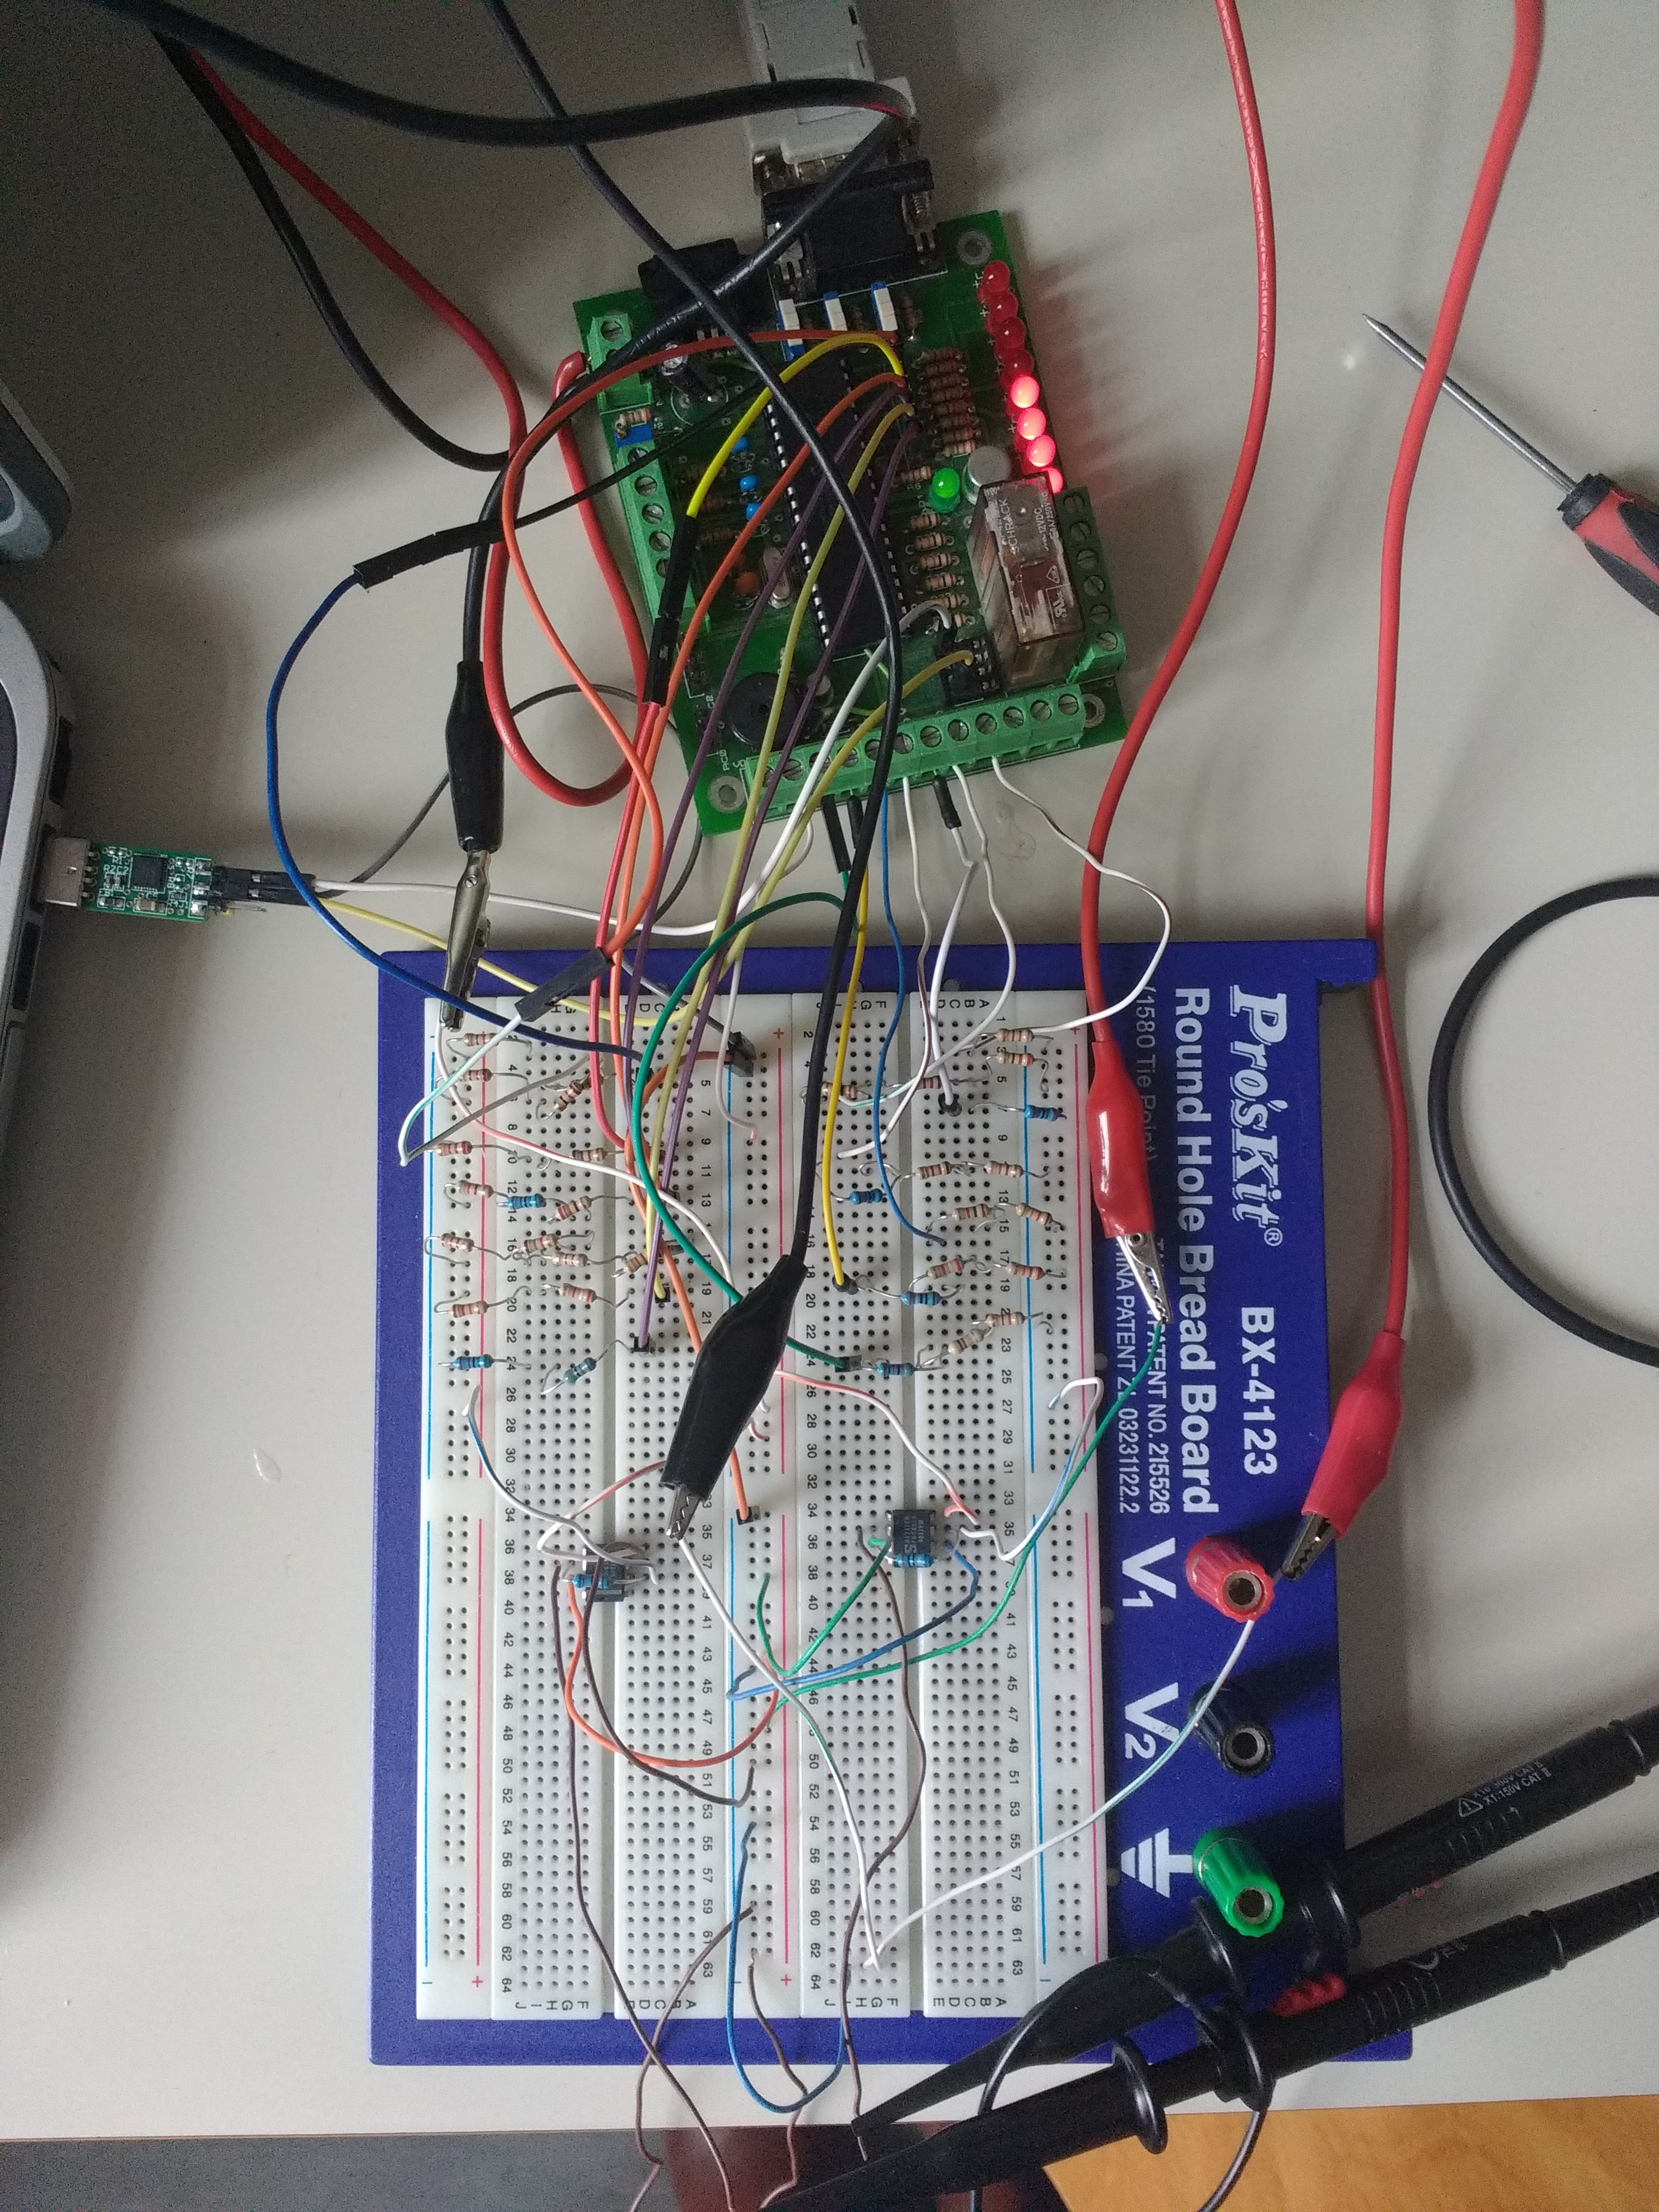
\includegraphics[scale=0.07]{shemaSPajanja.jpg}
  \caption{Shema spajanja}
  \label{fig:glavnasemalive}
\end{figure}
\newline

Serijska komunikacija je realizovana putem prekida. Kada se završi komunikacija na našem mikrokontroleru bude sačuvana matrica koja ima sljedeći oblik:
$
t\_byte$ $slika[40][5]= \{
\{  0b11111111, 0b00000000, 0b00000000, 0b00000000, 0b00000000\},\\
\{  0b00000000, 0b00000000, 0b00000000, 0b00000000, 0b00000000\},\\
\{  0b00000000, 0b00000000, 0b00000000, 0b00000000, 0b00000000\},\\
\{  0b00000000, 0b00000000, 0b00000000, 0b00000000, 0b00000000\},\\
\{  0b00000000, 0b00000000, 0b00000000, 0b00000000, 0b00000000\},\\
\{  0b11111111, 0b00000000, 0b00000000, 0b00000000, 0b00000000\},\\
\{  0b00000000, 0b00000000, 0b00000000, 0b00000000, 0b00000000\},\\
\{  0b00000000, 0b00000000, 0b00000000, 0b00000000, 0b00000000\},\\
\{  0b00000000, 0b00000000, 0b00000000, 0b00000000, 0b00000000\},\\
\{  0b00000000, 0b00000000, 0b00000000, 0b00000000, 0b00000000\},
...,
\};
$
\newline
\newline
Nakon prijema slike, vrši se prikazivanje iste do sljedećeg prekida odnosno dok korisnik ne zatraži prikaz nove slike.
Bitno je napomenuti da je prikaz slike programiran tako da se prikaže jedan red slike sa lijeva ka desnu, a naredni red se prikazuje sa desna ka lijevu. Razlog tome je da se ne prekida snop svjetlosti koji prikazuje slku prelaskom na novi red, već da ide "cik-cak". Posmatrajući matricu koja se formira treba istaći da bit "1" na osciloskopu predtsavlja postojanje piksela, a bit "0" obrnuto.\newline
Kakvu ulogu u svemu igraju digitalno-analogni konvertori? Naime, kako se obradjuje matrica bit po bit, i za svaki bit koji postavljen tj. ima vrijednost "1" odredjene vriejdnsoti se pojavljuju na PORTB i PORTD. Npr. ako je prvi bit u matrici postavljen tada će se na portovima PORTB i PORTD prikazati vrijednost 0. Ako je drugi bit postavljen na 1, onda će na PORTB biti vrijednost 0 (y koordinata) a na PORTD vrijednost 1+const (x koordinata). Kada se predje na naredni red matrice tada se mijenja i vrijednost na PORTB.\newline
Listing koda programiran na PIC16F1939 je prikazan u nastavku. 
\lstinputlisting[language=Octave]{ckod.txt}

\pagebreak
\section{EKSPERIMENTALNI REZULTATI}
U ovom poglavlju će biti prikazani rezultati dobiveni sa prikazom određenih slika. NAPOMENA: Sljedeće slike su uređene jer nije bilo moguće slikati čitavu sliku na osciloskpu iz tehničkih razloga. \newline
Na slikama \ref{fig:gui}, \ref{fig:gljivica}, \ref{fig:gui2}, \ref{fig:stop}, \ref{fig:gui3}, \ref{fig:srce}, \ref{fig:gui4} i \ref{fig:pa} su prikazani izgled prozora u Matlab-u i slike na osciloskopu.
\begin{figure}[h!]
    \centering
  \includegraphics[scale=0.4]{izgledGUIa.png}
  \caption{Izgled GUI-a Matlab}
  \label{fig:gui}
\end{figure}
\begin{figure}[h!]
    \centering
  \includegraphics[scale=1.55]{gljivica3.jpg}
  \caption{Prikaz slike na osciloskopu}
  \label{fig:gljivica}
\end{figure}

\begin{figure}[h!]
    \centering
  \includegraphics[scale=0.4]{51216169_2121010267980352_2222276474780516352_n.png}
  \caption{Izgled GUI-a Matlab}
  \label{fig:gui2}
\end{figure}
\begin{figure}[h!]
    \centering
  \includegraphics[scale=0.5]{stopfinal.jpg}
  \caption{Prikaz slike na osciloskopu}
  \label{fig:stop}
\end{figure}



\begin{figure}[h!]
    \centering
  \includegraphics[scale=0.4]{51427942_1953607828071413_2929664988660367360_n.png}
  \caption{Izgled GUI-a Matlab-a}
  \label{fig:gui3}
\end{figure}
\begin{figure}[h!]
    \centering
  \includegraphics[scale=0.5]{srcefinal.jpg}
  \caption{Prikaz slike na osciloskopu}
  \label{fig:srce}
\end{figure}
\begin{figure}[h!]
    \centering
  \includegraphics[scale=0.4]{51558858_373678219851352_3569912928796672000_n.png}
  \caption{Izgled GUI-a Matlab-a}
  \label{fig:gui4}
\end{figure}

\begin{figure}[h!]
    \centering
  \includegraphics[scale=0.70]{PAfinal.jpg}
  \caption{Prikaz slike na osciloskopu}
  \label{fig:pa}
\end{figure}
\newline
Na slikama \ref{fig:adap} i \ref{fig:glp} je prikazana razlika izmedju neadaptivnog i adaptivnog procesiranja slike.
\begin{figure}[h!]
    \centering
  \includegraphics[scale=0.65]{50853112_240538963524513_8617086812604596224_n.png}
  \caption{Adaptivno procesiranje slike}
  \label{fig:adap}
\end{figure}
\begin{figure}[h!]
    \centering
  \includegraphics[scale=0.65]{51223868_2219858701618201_6484712911091531776_n.png}
  \caption{Neadaptivno procesiranje slike}
  \label{fig:glp}
\end{figure}
\pagebreak

\section{ZAKLJUČAK}
Projekat smo realizirali na osnovu prethodno stečenog znanja iz predmeta Praktikum
Automatike, ali i predmeta Ugradbeni sistemi. Također, bilo je potrebno dodatno upoznavanje sa
funkcijama mikrokontrolera jer na laboratorijskim vježbama nije rađena serijska komunikacija. Glavni cilj bio je
teoretsko shvatanje pozadine koja se dešava iza samog ekrana osciloskopa tj. kako doći do
prikaza slike. Kako smo izabrali da za prikaz slike koristimo dva digitalno-analogna konvertora bilo je potrebno dodatno prouciti samo implementaciju istih. Najveći problem predstavlja slanje signala na osciloskop jer razvojni sistem nije dovoljno brz da bi uspio prikazati sve piksele a da to ljudsko oko posmatra kao jednu sliku.
\pagebreak
\section{LITERATURA}

\begin{itemize}
  \item Dokumentacija za mikrokontroler Microchip PIC16F1939 
  \item Praktikum automatike i elektronike (Skripta - radna verzija) - M. Kuric, S. Konjicija & A. Aksamovic
\item Praktikum automatike – predavanje za ak.god. 2018/2019 \\
Vanr. prof. dr Samim Konjicija, dipl. ing. el.\\
Vanr. prof. dr Abdulah Akšamović, dipl. ing. el.


\end{itemize}
\pagebreak
\phantomsection 
\addcontentsline{toc}{chapter}{Bibliography} 
\bibliographystyle{unsrtnat} 
\bibliography{fyp}

\end{document}